% ===== k-means =====
\section*{K-Means Clustering}
% ---- CS189 scope checklist: must include ([x] = already covered) ----
% Source: Lecture 2; reference sheet p.4
% [x] Goal: split N points into K clusters; K is a hyperparameter
% [x] Objective: sum of squared distances to own center
% [x] Lloyd's algorithm: assign to nearest center, move center to cluster mean
% [x] Always converges, but to a local minimum; rerun with random starts
% [x] Choosing K: domain knowledge, elbow method
% [ ] Clusters are not labels: they depend on the features chosen
% [ ] Recognize the sheet's one-hot notation r_nk (same as your z_n)
% ----

\subsection*{What Clustering Does}
\textbf{Goal:} split the data into $K$ groups (clusters) of points that are close together. In the unsupervised plot, an algorithm should discover the 2 groups on its own.
\begin{itemize}
  \item \textbf{Most common use: market segmentation.} Given a database of customers, group them by e.g.\ age/gender so each group can get its own marketing campaign.
  \item The first clustering algorithm is \textbf{K-means}. $K$ = number of clusters (a hyperparameter we pick).
\end{itemize}

\subsection*{K-Means (Lloyd's Algorithm)}
\textbf{Notation.}
\begin{itemize}
  \item $\boldsymbol{\mu}_k \in \mathbb{R}^D$: the \textbf{cluster center} (centroid) of cluster $k$, for $k = 1, \dots, K$. These are the crosses.
  \item $z_n \in \{1, \dots, K\}$: the \textbf{assignment} of point $\mathbf{x}_n$, i.e.\ which cluster (color) it belongs to.
\end{itemize}

\textbf{Step 0: Initialize.} Pick $K$ starting centers $\boldsymbol{\mu}_1, \dots, \boldsymbol{\mu}_K$ at random (common choice: $K$ random training points).

\textbf{Then repeat (K-means is iterative):}

\textbf{Step 1: Update assignments.} Go through every training example and color it by whichever center is closest:
\[
z_n = \arg\min_{k} \; \|\mathbf{x}_n - \boldsymbol{\mu}_k\|_2^2
\qquad \text{for every } n = 1, \dots, N
\]

\textbf{Step 2: Update centers.} Move each cross to the mean (centroid) of the points with its color:
\[
\boldsymbol{\mu}_k = \frac{1}{N_k} \sum_{n \,:\, z_n = k} \mathbf{x}_n
\qquad N_k = \text{number of points assigned to cluster } k
\]

\subsection*{Example: $K = 2$}
Same 12 points as the unsupervised plot:

{\centering
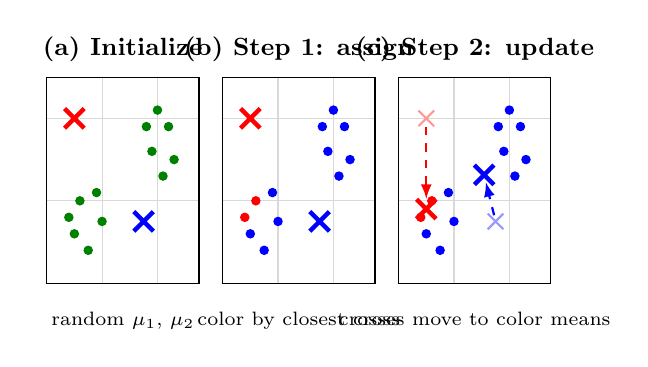
\begin{tikzpicture}
% ---- (a) initialize ----
\begin{axis}[name=k0,
    width=0.29\linewidth, height=4.2cm,
    xmin=0, xmax=5.5, ymin=0, ymax=5, enlargelimits=false,
    grid=major, grid style={gray!30}, major tick length=0pt,
    xticklabels={}, yticklabels={},
    title={\small\textbf{(a) Initialize}}, title style={yshift=-4pt},
    xlabel={\scriptsize random $\boldsymbol{\mu}_1$, $\boldsymbol{\mu}_2$}, label style={font=\scriptsize}]
\addplot[only marks, mark=*, green!50!black, mark size=1.5pt] coordinates {(1,1.2) (1.5,0.8) (2,1.5) (1.2,2) (1.8,2.2) (0.8,1.6) (3.8,3.2) (4.4,3.8) (4,4.2) (4.6,3) (3.6,3.8) (4.2,2.6)};
\addplot[only marks, mark=x, red, mark size=5pt, ultra thick] coordinates {(1,4)};
\addplot[only marks, mark=x, blue, mark size=5pt, ultra thick] coordinates {(3.5,1.5)};
\end{axis}
% ---- (b) assign ----
\begin{axis}[name=k1, at={(k0.east)}, anchor=west, xshift=0.3cm,
    width=0.29\linewidth, height=4.2cm,
    xmin=0, xmax=5.5, ymin=0, ymax=5, enlargelimits=false,
    grid=major, grid style={gray!30}, major tick length=0pt,
    xticklabels={}, yticklabels={},
    title={\small\textbf{(b) Step 1: assign}}, title style={yshift=-4pt},
    xlabel={\scriptsize color by closest cross}, label style={font=\scriptsize}]
\addplot[only marks, mark=*, red, mark size=1.5pt] coordinates {(1.2,2) (0.8,1.6)};
\addplot[only marks, mark=*, blue, mark size=1.5pt] coordinates {(1,1.2) (1.5,0.8) (2,1.5) (1.8,2.2) (3.8,3.2) (4.4,3.8) (4,4.2) (4.6,3) (3.6,3.8) (4.2,2.6)};
\addplot[only marks, mark=x, red, mark size=5pt, ultra thick] coordinates {(1,4)};
\addplot[only marks, mark=x, blue, mark size=5pt, ultra thick] coordinates {(3.5,1.5)};
\end{axis}
% ---- (c) update ----
\begin{axis}[name=k2, at={(k1.east)}, anchor=west, xshift=0.3cm,
    width=0.29\linewidth, height=4.2cm,
    xmin=0, xmax=5.5, ymin=0, ymax=5, enlargelimits=false,
    grid=major, grid style={gray!30}, major tick length=0pt,
    xticklabels={}, yticklabels={},
    title={\small\textbf{(c) Step 2: update}}, title style={yshift=-4pt},
    xlabel={\scriptsize crosses move to color means}, label style={font=\scriptsize}]
\addplot[only marks, mark=*, red, mark size=1.5pt] coordinates {(1.2,2) (0.8,1.6)};
\addplot[only marks, mark=*, blue, mark size=1.5pt] coordinates {(1,1.2) (1.5,0.8) (2,1.5) (1.8,2.2) (3.8,3.2) (4.4,3.8) (4,4.2) (4.6,3) (3.6,3.8) (4.2,2.6)};
\addplot[only marks, mark=x, red!40, mark size=4pt, thick] coordinates {(1,4)};
\addplot[only marks, mark=x, blue!40, mark size=4pt, thick] coordinates {(3.5,1.5)};
\addplot[red, thick, dashed, -latex] coordinates {(1,3.8) (1,2.05)};
\addplot[blue, thick, dashed, -latex] coordinates {(3.45,1.65) (3.15,2.45)};
\addplot[only marks, mark=x, red, mark size=5pt, ultra thick] coordinates {(1.0,1.8)};
\addplot[only marks, mark=x, blue, mark size=5pt, ultra thick] coordinates {(3.09,2.63)};
\end{axis}
\end{tikzpicture}

\vspace{4pt}
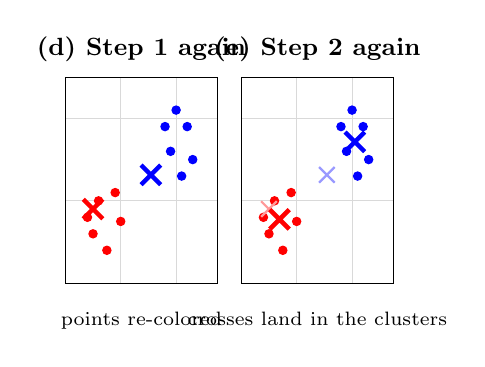
\begin{tikzpicture}
% ---- (d) assign again ----
\begin{axis}[name=k3,
    width=0.29\linewidth, height=4.2cm,
    xmin=0, xmax=5.5, ymin=0, ymax=5, enlargelimits=false,
    grid=major, grid style={gray!30}, major tick length=0pt,
    xticklabels={}, yticklabels={},
    title={\small\textbf{(d) Step 1 again}}, title style={yshift=-4pt},
    xlabel={\scriptsize points re-colored}, label style={font=\scriptsize}]
\addplot[only marks, mark=*, red, mark size=1.5pt] coordinates {(1,1.2) (1.5,0.8) (2,1.5) (1.2,2) (1.8,2.2) (0.8,1.6)};
\addplot[only marks, mark=*, blue, mark size=1.5pt] coordinates {(3.8,3.2) (4.4,3.8) (4,4.2) (4.6,3) (3.6,3.8) (4.2,2.6)};
\addplot[only marks, mark=x, red, mark size=5pt, ultra thick] coordinates {(1.0,1.8)};
\addplot[only marks, mark=x, blue, mark size=5pt, ultra thick] coordinates {(3.09,2.63)};
\end{axis}
% ---- (e) update again ----
\begin{axis}[name=k4, at={(k3.east)}, anchor=west, xshift=0.3cm,
    width=0.29\linewidth, height=4.2cm,
    xmin=0, xmax=5.5, ymin=0, ymax=5, enlargelimits=false,
    grid=major, grid style={gray!30}, major tick length=0pt,
    xticklabels={}, yticklabels={},
    title={\small\textbf{(e) Step 2 again}}, title style={yshift=-4pt},
    xlabel={\scriptsize crosses land in the clusters}, label style={font=\scriptsize}]
\addplot[only marks, mark=*, red, mark size=1.5pt] coordinates {(1,1.2) (1.5,0.8) (2,1.5) (1.2,2) (1.8,2.2) (0.8,1.6)};
\addplot[only marks, mark=*, blue, mark size=1.5pt] coordinates {(3.8,3.2) (4.4,3.8) (4,4.2) (4.6,3) (3.6,3.8) (4.2,2.6)};
\addplot[only marks, mark=x, red!40, mark size=4pt, thick] coordinates {(1.0,1.8)};
\addplot[only marks, mark=x, blue!40, mark size=4pt, thick] coordinates {(3.09,2.63)};
\addplot[only marks, mark=x, red, mark size=5pt, ultra thick] coordinates {(1.38,1.55)};
\addplot[only marks, mark=x, blue, mark size=5pt, ultra thick] coordinates {(4.1,3.43)};
\end{axis}
\end{tikzpicture}
\par}

\subsection*{Cost Function}
Total squared distance from each point to its own center. K-means finds the $z$ and $\boldsymbol{\mu}$ that minimize it:
\[
J(z, \boldsymbol{\mu}) = \sum_{n=1}^{N} \|\mathbf{x}_n - \boldsymbol{\mu}_{z_n}\|_2^2
\]
\begin{itemize}
  \item Small $J$ = tight clusters. E.g.\ points $1, 2, 9, 10$: clusters $\{1,2\},\{9,10\}$ give $J = 1$; clusters $\{1\},\{2,9,10\}$ give $J = 38$.
  \item Step 1 lowers $J$ by changing the colors $z$; Step 2 lowers $J$ by moving the centers $\boldsymbol{\mu}$.
  \item \textbf{Converges:} each step can only lower $J$ (or keep it the same), and $J \geq 0$, so $J$ settles at a final value.
  \item \textbf{Local minima:} that final value depends on the starting centers. Fix: run K-means several times with different random starts and keep the lowest $J$.
\end{itemize}

\subsection*{Choosing $K$}
The right number of clusters is often ambiguous. Don't just minimize $J$: it always shrinks as $K$ grows ($K = N \Rightarrow J = 0$).
\begin{itemize}
  \item \textbf{Domain understanding:} e.g.\ 3 penguin species $\Rightarrow K = 3$; 4 marketing campaigns $\Rightarrow K = 4$.
  \item \textbf{Elbow method:} plot $J$ vs.\ $K$ and pick where the improvement levels off.
\end{itemize}

{\centering
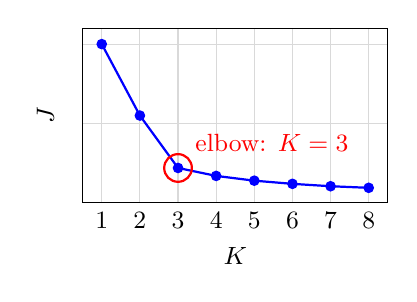
\begin{tikzpicture}
\begin{axis}[
    width=0.45\linewidth, height=3.8cm,
    xmin=0.5, xmax=8.5, ymin=0, ymax=110, enlargelimits=false,
    grid=major, grid style={gray!30}, major tick length=0pt,
    xtick={1,...,8}, yticklabels={},
    xlabel={$K$}, ylabel={$J$},
    tick label style={font=\small}, label style={font=\small}]
\addplot[thick, blue, mark=*, mark size=1.5pt] coordinates {(1,100) (2,55) (3,22) (4,17) (5,14) (6,12) (7,10.5) (8,9.5)};
\addplot[only marks, mark=o, red, mark size=5pt, thick] coordinates {(3,22)};
\node[font=\small, red, anchor=south west] at (axis cs:3.2,26) {elbow: $K = 3$};
\end{axis}
\end{tikzpicture}
\par}
